\chapter{Proposed System}
\section{Introduction}
This chapter will present our proposed system as the solution. We will define our system and show how it solves the problem of maintaining privacy for the users.
\section{User Identification}
In order to solve the problem we first look at how the users are identified in the system. There are 2 ways by which bank can identify the actual users
\begin{itemize}
	\item From the logs i.e. transaction data
\\
\\Banks store all the logs or transaction data with real id of the user. Its easy to access this data by the bank for a given user and extract all of his data.
	\item From a database in the bank system where personal details of the user are stored.	
\\
\\Bank stores personal data about all its users in a database. As this database lies at the bank, its possible for bank to use the database to get the personal information about a user.
\end{itemize}
We can remove this identification in following ways.
\begin{itemize}
	\item Remove the user identity from the logs and transaction data
\\
\\This way there is no way for the bank to get transaction data for a given user as there will be no user identity linked to the logs or transactions.
	\item Either remove the user personal data or limit the access to this personal database
\\
\\If bank removes the personal database of the users from its side, then there is no way bank can get personal information of the users.
\\
\\If bank limit access to such database and don't really use it for day to day banking purposes then its also possible for bank to limit access to user personal information.
\end{itemize}
\section{Pseudonym System}
In order to provide privacy to the users, we suggest a new pseudonym system.
\begin{figure}[h]
\centering
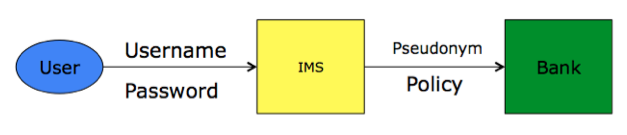
\includegraphics[width=\textwidth]{figures/Pseudonym}
\caption{Pseudonym Banking System}
\label{fig:Pseudonym}
\end{figure}
In our system we modify the Authentication service and replace it with an Identity Mapping System (IMS)
\begin{itemize}
	\item Instead of giving the User ID to the bank we actually replace it with a pseudonym
	\item The IMS sends the policy as well as account ID to the bank	
	\item Bank then use this information to provide service to the customer
	\item Bank doesn’t need to store the mapping databases
\end{itemize}
The IMS can either be in the bank in a separate department or a 3rd party can manage it. This way the bank doesn’t need to know the exact identity of the user to provide them with the services.
Also bank can still store personal details of the user in case of legal requirement but it can be stored at a separate place as its not needed for day to day operation of the bank.
\section{Properties}
Following privacy properties are desirable in our pseudonym system.
\begin{itemize}
	\item \textbf{Unlinkability} If the same pseudonym is used with different identities or different pseudonyms are used for same identity it should not be possible to link these different transactions to the same person. 
	\item \textbf{Partial Information Disclosure} The information given by a user should be minimum and he should be able to choose what information values it actually wants to be made available to the bank. 
	\item \textbf{Conditional Anonymity Removal} In case of some discrepancy or legal requirement, the authorities should be able to come in and identify the real user from the Pseudonym.
	\item \textbf{Revocation} It should be easy to revoke any user. Also it should be easy to check whether a certain user is revoked or not. 
\end{itemize}
\section{User Privacy}
As in our system bank never gets the real identity of the user, the user anonymity to the bank is maintained. Also bank doesn't need to store the policies for the users as its all coming from the IMS. As a result, it decreases a lot of load from the bank to store such data. IMS service adds a layer of pseudonymity in the system. 

\section{Summary}
In this chapter we presented our pseudonym system. Also we have given some certain privacy properties that our pseudonym system should be able to fulfill. In the next chapter, we will discuss about the prototype with the pseudonym system.
\\
\\For our purposes we have decided to take case of 2 different systems for our IMS
\begin{itemize}
	\item OpenID
	\item IDEMIX
\end{itemize}